\chapter{An Example: The Nim Game}
\label{cha:the-nim-game}


This chapter contains a full example program that can give you
some basic idea of using the simulator. An enhanced version of
the Nim example can be found among the sample programs.

Nim is an ancient game with two players and a bunch of sticks.
The players take turns, removing 1, 2, 3 or 4 sticks from the
heap of sticks at each turn. The one who takes the last stick
is the loser.


Of course, building a model of the Nim game is not much of a
simulation project, but it nicely demonstrates the modeling approach
used by {\opp}.


Describing the model consists of two phases:
\begin{itemize}
\item{topology description}
\item{defining the operation of components}
\end{itemize}



\section{Topology}

The game can be modelled in {\opp} as a network with three modules:
the ``game'' (a manager module) and two players.
The modules will communicate by exchanging messages. The ``game''
module keeps the current number of tokens and organizes the game;
in each turn, the player modules receives the number of tokens
from the Game module and sends back its move.

\begin{figure}[htbp]
\begin{center}
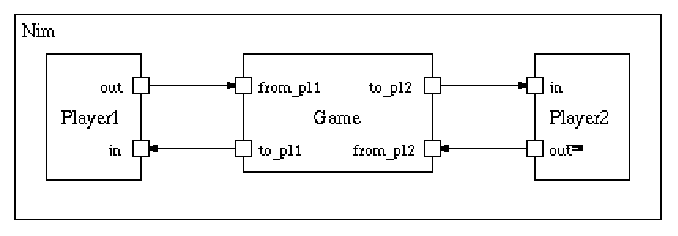
\includegraphics[width=4.483in, height=1.568in]{figures/usmanFig6}
\caption{Module structure for the Nim game.}
\end{center}
\end{figure}

\texttt{Player1}, \texttt{Player2} and \texttt{Game} are simple
modules (e.g. they have no submodules.) Each module is an instance of
a module type. We'll need a module type to represent the \texttt{Game} module;
let's call it \texttt{Game} too.

We can implement two kinds of players: \texttt{SmartPlayer}, which knows
the winning algorithm, and \texttt{SimplePlayer}, which simply takes a
random number of sticks. In our example, \texttt{Player1} will be a \texttt{SmartPlayer}
and \texttt{Player2} will be a \texttt{SimplePlayer}.

The enclosing module, \texttt{Nim} is a compound module (it has submodules).
It is also defined as a module type of which one instance is
created, the system module.

Modules have input and output gates\index{gate} (the tiny boxes
labeled \texttt{in}, \texttt{out}, \texttt{fromPlayer1}, etc. in the
figure). An input and an output gate can be connected: connections (or
links) are shown as in the figure as arrows.  During the simulation,
modules communicate by sending messages through the connections.


The user defines the topology\index{topology!defining} of the network in NED files\index{ned!files}.


We placed the model description in two files; the first file
defines the simple module types and the second one the system
module.

The first file (NED keywords are typed in boldface):

\begin{Verbatim}[commandchars=\\\{\}]
//---------------------------------------------------------
// file: nim_mod.ned
// Simple modules in nim.ned
//---------------------------------------------------------


// Declaration of simple module type Game.

\textbf{simple} Game
    \textbf{parameters}:
         numSticks, // initial number of sticks
         firstMove; // 1=Player1, 2=Player2

    \textbf{gates}:
        \textbf{in}:
             fromPlayer1, // input and output gates
             fromPlayer2; // for connecting to Player1/Player2
        \textbf{out}:
             toPlayer1,
             toPlayer2;
\textbf{endsimple}


// Now the declarations of the two simple module types.
// Any one of the two types can be Player1 or Player2.

// A player that makes random moves
\textbf{simple} SimplePlayer
    \textbf{gates}:
        \textbf{in}: in; // gates for connecting to Game
        \textbf{out}: out;
\textbf{endsimple}

// A player who knows the winning algorithm
\textbf{simple} SmartPlayer
    \textbf{gates}:
        \textbf{in}: in; // gates for connecting to Game
        \textbf{out}: out;
\textbf{endsimple}
\end{Verbatim}

The second file:

\begin{Verbatim}[commandchars=\\\{\}]
//-------------------------------------------------------------
// file: nim.ned
// Nim compound module + system module
//-------------------------------------------------------------

\textbf{import} "nim_mod";

\textbf{module} Nim
    \textbf{submodules}:
        game: Game
            \textbf{parameters}:
                numSticks = intuniform(21, 31),
                firstMove = intuniform(1, 2);
        player1: SmartPlayer;
        player2: SimplePlayer;
    \textbf{connections}:
        player1.out --> game.fromPlayer1,
        player1.in <-- game.toPlayer1,
        player2.out --> game.fromPlayer2,
        player2.in <-- game.toPlayer2;
\textbf{endmodule}

// system module creation
\textbf{network}
    nim: Nim
\textbf{endnetwork}
\end{Verbatim}



\section{Simple modules}

The module types \texttt{SmartPlayer}, \texttt{SimplePlayer} and \texttt{Game} are implemented
in C++, using the {\opp} library classes and functions.

Each simple\index{module!simple} module type is derived from the C++
class \cclass{cSimpleModule}, with its \fname{activity()} member
function redefined. The \fname{activity()} functions of all
simple\index{module!simple} modules in the network are executed as
coroutines\index{coroutine}, so they appear as if they were running in
parallel.  Messages are instances of the class \cclass{cMessage}.

We present here the C++ sources of the \texttt{SmartPlayer} and \texttt{Game} module
types.

The \texttt{SmartPlayer} first introduces himself by sending its name
to the \texttt{Game} module. Then it enters an infinite loop; with each
iteration, it receives a message from \texttt{Game} with the number of
sticks left, it calculates its move and sends back a message
containing the move.

Here's the source:

\begin{verbatim}
#include <stdio.h>
#include <string.h>
#include <time.h>

#include <omnetpp.h>

// derive SmartPlayer from cSimpleModule
class SmartPlayer : public cSimpleModule
{
    Module_Class_Members( SmartPlayer, cSimpleModule, 8192)
    // this is a macro; it expands to constructor definition etc.
    // 8192 is the size for the coroutine stack (in bytes)

virtual void activity();
    // this redefined virtual function holds the algorithm
};

// register the simple module class to OMNeT++
Define_Module( SmartPlayer );

// define operations of SmartPlayer
void SmartPlayer::activity()
{
    int move;

    // initialization phase: send module type to Game module
    // create a message with the name "SmartPlayer" and send it to Game

    cMessage *msg = new cMessage("SmartPlayer");
    send(msg, "out");

    // infinite loop to process moves;
    // simulation will be terminated by Game

    for (;;)
    {
        // messages have several fields; here, we'll use the message
        // kind member to store the number of sticks
        cMessage *msgin = receive();    // receive message from Game
        int numSticks = msgin->kind();  // extract message kind (an int)
                                        // it hold the number of sticks
                                        // still on the stack
        delete msgin;                   // dispose of the message

        move = (numSticks + 4) % 5;     // calculate move
        if (move == 0)                  // we cannot take zero
            move = 1;                   // seems like we going to lose

        ev << "Taking " << move         // some debug output. The ev
           << " out of " << numSticks   // object represents the user
           << " sticks.\n";             // interface of the simulator

        cMessage *msgout = new cMessage;// create empty message
        msgout->setKind( move );        // use message kind as storage
                                        // for move
        send( msgout, "out"); // send the message to Game
    }
}
\end{verbatim}

The \texttt{Game} module first waits for a message from both players
and extracts the message names that are also the players' names.  Then
it enters a loop, with the \texttt{playerToMove} variable
alternating between 1 and 2. With each iteration, it sends out a
message with the current number of sticks to the corresponding player
and gets back the number of sticks taken by that player. When the
sticks are out, the module announces the winner and ends the
simulation.

The source:


\begin{verbatim}
//-------------------------------------------------------------
// file: game.cc
// (part of NIM - an OMNeT++ demo simulation)
//-------------------------------------------------------------

#include <stdio.h>
#include <string.h>

#include <omnetpp.h>

// derive Game from cSimpleModule
class Game : public cSimpleModule
{
    Module_Class_Members(Game,cSimpleModule,8192)
      // this is a macro; it expands to constructor definition etc.
      // 8192 is the size for the coroutine stack (in bytes)

    virtual void activity();
      // this redefined virtual function holds the algorithm
};

// register the simple module class to OMNeT++
Define_Module( Game );

// operation of Game:
void Game::activity()
{
    // strings to store player names; player[0] is unused
    char player[3][32];

    // read parameter values
    int numSticks = par("numSticks");
    int playerToMove = par("firstMove");

    // waiting for players to tell their names
    for (int i=0; i<2; i++)
    {
        cMessage *msg = receive();
        if (msg->arrivedOn("fromPlayer1"))
            strcpy( player[1], msg->name());
        else
            strcpy( player[2], msg->name());
        delete msg;
    }

    // ev represents the user interface of the simulator
    ev << "Let the game begin!\n";
    ev << "Player 1: " << player[1] << "   Player 2: " << player[2]
       << "\n\n";

    do
    {
        ev << "Sticks left: " << numSticks << "\n";
        ev << "Player " << playerToMove << " ("
           << player[playerToMove] << ") to move.\n";

        cMessage *msg = new cMessage("", numSticks);
                        // numSticks will be the msg kind

        if (playerToMove == 1)
            send(msg, "toPlayer1");
        else
            send(msg, "toPlayer2");

        msg = receive();
        int sticksTaken = msg->kind();
        delete msg;

        numSticks -= sticksTaken;

        ev << "Player " << playerToMove << " ("
           << player[playerToMove] << ") took "
           << sticksTaken << " stick(s).\n";

        playerToMove = 3 - playerToMove;
    }
    while (numSticks>0);

    ev << "\nPlayer " << playerToMove << " ("
       << player[playerToMove] << ") won!\n";

    endSimulation();
}
\end{verbatim}




\section{Running the simulation}

Once the source files are ready, one needs to compile and link
them into a simulation executable. One can specify the user interface
to be linked.

Before running the simulation, one can put parameter values and
all sorts of other settings into an initialization file that
will be read when the simulation program starts\index{simulation!configuration}:

\index{omnetpp.ini}

\begin{verbatim}
#
# file: omnetpp.ini
#

[General]
network = nim
random-seed = 3
ini-warnings = false

[Cmdenv]
express-mode = no
\end{verbatim}

Suppose we link the Nim simulation with the command line user
interface. We get the executable \ttt{nim} (\ttt{nim.exe} under Windows).
When we run it, we'll get the following screen output:

\begin{verbatim}
% ./nim
\end{verbatim}

Or:

\begin{verbatim}
C:\OMNeT++\samples\nim> nim

OMNeT++ Discrete Event Simulation  (C) 1992-2003 Andras Varga
See the license for distribution terms and warranty disclaimer
Setting up Cmdenv (command-line user interface)...

Preparing for Run #1...
Setting up network `nim'...
Running simulation...

Let the game begin!
Player 1: SmartPlayer Player 2: SimplePlayer

Sticks left: 29
Player 2 (SimplePlayer) to move.
SimplePlayer is taking 2 out of 29 sticks.
Player 2 (SimplePlayer) took 2 stick(s).
Sticks left: 27
Player 1 (SmartPlayer) to move.
SmartPlayer is taking 1 out of 27 sticks.
Player 1 (SmartPlayer) took 1 stick(s).
Sticks left: 26
[...]
Sticks left: 5
Player 1 (SmartPlayer) to move.
SmartPlayer is taking 4 out of 5 sticks.
Player 1 (SmartPlayer) took 4 stick(s).
Sticks left: 1
Player 2 (SimplePlayer) to move.
SimplePlayer is taking 1 out of 1 sticks.
Player 2 (SimplePlayer) took 1 stick(s).

Player 1 (SmartPlayer) won!
<!> Module nim.game: Simulation stopped with endSimulation().

End run of OMNeT++
\end{verbatim}



\section{Other examples}

An enhanced version of the Nim example can be found among the sample
programs. It adds a third, interactive player and derives specific
player types from a \texttt{Player} abstract class. It also adds the
possibility that actual types for \texttt{player1} and
\texttt{player2} can be specified in the ini file or interactively
entered by the user at the beginning of the simulation.

Nim does not show very much of how complex algorithms like communication
protocols can be implemented in {\opp}. To have an idea about
that, look at the Token Ring example. It is also extensively
commented, though you may need to peep into the user manual to
fully understand it. The Dyna simulation models a simple
client-server network and demonstrates dynamic module creation.
The FDDI example is an accurate FDDI MAC simulation
which was written on the basis of the ANSI standard.


The following table summarizes the sample simulations:

\begin{longtable}{|l|p{4.2cm}|p{8cm}|}
\hline
\tabheadcol
\textbf{NAME} & \textbf{TOPIC} & \textbf{DEMONSTRATES}\\\hline
% ROW 2
\textbf{nim} & a simple two-player game
&
{\raggedright module inheritance;
module type as parameter}\\\hline
% ROW 3
\textbf{hcube}
&
{\raggedright hypercube network with deflection routing}
&
{\raggedright hypercube topology with dimension as parameter;
topology templates;
output vectors}\\\hline
% ROW 4
\textbf{token} & Token Ring network
&
{\raggedright ring topology with the number of nodes as parameter;
using \cclass{cQueue};
\fname{wait()};
output vectors}\\\hline
% ROW 5
\textbf{fifo1} & single-server queue
&
{\raggedright simple module inheritance;
decomposing \fname{activity()} into several functions;
using simple statistics and output vectors;
printing stack usage info to help optimize memory consumption;
using \fname{finish()}}\\\hline
% ROW 6
\textbf{fifo2} & another fifo implementation
&
{\raggedright using \ttt{handleMessage()};
decomposing \texttt{handleMessage()} into several functions;
the FSM macros;
simple module inheritance;
using simple statistics and output vectors;
using \texttt{finish()}}\\\hline
% ROW 7
\textbf{fddi} & FDDI MAC simulation
&
{\raggedright using statistics classes;
and many other features}\\\hline
% ROW 8
\textbf{hist} & demo of the histogram classes
&
{\raggedright collecting observations into statistics objects;
saving statistics objects to file and restoring them}\\\hline
% ROW 9
\textbf{dyna} & a client-server network
&
{\raggedright dynamic module creation;
using \fmac{WATCH()};
star topology with the number of modules as parameters}\\\hline
% ROW 10
\textbf{topo} & various topologies
&
{\raggedright using NED for creating parametrized topologies}\\\hline
% ROW 11
\textbf{demo} & tour of {\opp} samples & shows how to link several sim. models into one executable\\\hline
\end{longtable}


%%% Local Variables:
%%% mode: latex
%%% TeX-master: "usman"
%%% End:
